% p10-06 例 1：正方形 ABCD 边长 a=6（具体值），E∈BC, F∈CD, ∠EAF=45°，证 EF=BE+DF
% 把 △ABE 绕 A 顺时针 90° → △ADE'，E' 在 CD 延长线
% A(0,6), B(6,6), C(6,0), D(0,0)  —— 让 BE 在右、DF 在下
% 顺时针 90° 绕 A：(x,y)−A → (y-Ay, -(x-Ax))+A   即 P-A → (P.y-A.y, -(P.x-A.x))
% B(6,6)-A=(6,0) → (0,-6) → B'=A+(0,-6)=(0,0)=D ✓
% 取示例 BE=2, DF=3 → EF=5 (在 Rt △CEF: CE=4, CF=3, EF=5 ✓)
\documentclass[tikz,border=4pt]{standalone}
\usepackage{ctex}
\usepackage{amsmath}
\usetikzlibrary{calc, arrows.meta}
\begin{document}
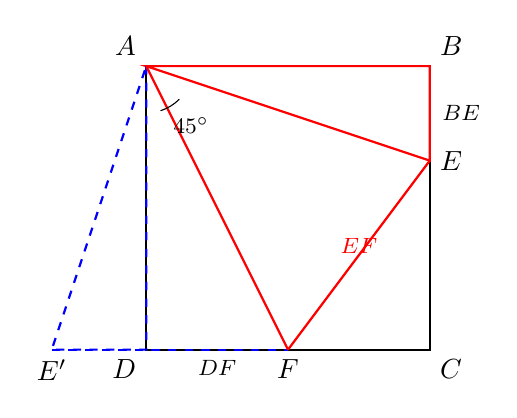
\begin{tikzpicture}[scale=0.6, thick]
  \coordinate (A) at (0,6);
  \coordinate (B) at (6,6);
  \coordinate (C) at (6,0);
  \coordinate (D) at (0,0);
  \coordinate (E) at (6,4);   % BE=2
  \coordinate (F) at (3,0);   % DF=3
  % E 顺时针 90° 绕 A：E-A=(6,-2) → (-2,-6) → E'=A+(-2,-6)=(-2,0)
  \coordinate (Ep) at (-2,0);

  \draw (A)--(B)--(C)--(D)--cycle;

  % △ABE
  \draw[red, thick] (A)--(B)--(E)--cycle;
  % △ADE' 旋转后 (E 在 CD 延长线)
  \draw[blue, dashed, thick] (A)--(D)--(Ep)--cycle;

  % 折线 EF + E'F (E'F = E'D + DF = 2 + 3 = 5 = EF ✓)
  \draw[red, thick] (E)--(F);
  \draw[blue, dashed, thick] (Ep)--(F);

  % AF (公共边)
  \draw[red, thick] (A)--(F);

  % 角标 ∠EAF=45°
  \draw[thin] ($(A)+(0.7,-0.7)$) arc[start angle=-45, end angle=-72, radius=1.0];
  \node[font=\footnotesize] at (0.95, 4.75) {$45^\circ$};

  \node[above left]  at (A) {$A$};
  \node[above right] at (B) {$B$};
  \node[below right] at (C) {$C$};
  \node[below left]  at (D) {$D$};
  \node[right] at (E) {$E$};
  \node[below] at (F) {$F$};
  \node[below] at (Ep) {$E'$};

  \node[font=\footnotesize, right] at (6.05, 5) {$BE$};
  \node[font=\footnotesize, below] at (1.5, 0) {$DF$};
  \node[font=\footnotesize, red] at (4.5, 2.2) {$EF$};
\end{tikzpicture}
\end{document}
